\section{模块间分析}\label{intermodule-analysis}

模块间分析是本文所设计的软件变更分析系统中最为重要的部分。AOSP 由若干仓库组成,各仓库又由若干模块组成,然而各仓库与模块并非完全封闭的。在构建时,某仓库下的模块可能会使用其他仓库下的另一模块,这导致单模块变动可能产生难以想象的影响。因此,对 AOSP 进行模块间分析是极其重要的。本节从 soong 的模块概念入手,扩展了有向图概念,提出了基于 AOSP 完全构建过程的模块间分析算法。

\subsection{soong 的模块概念}

soong 作为 Android Tiramisu 使用的顶层构建系统,继承了 Android Nought 以 GNU Make 为主导的构建系统下模块的概念,如图\ref{fig:aosp-3-layer}所示使用 “仓库-模块-文件” 三层为庞大的 AOSP 分级。

\begin{itemize}
    \item Google 使用 git 作为 AOSP 的版本控制系统,进而使得仓库成为 AOSP 最上层结构单元。
    \item soong 使用 Android.bp 对 AOSP 进行下一层分级。本文所设计的软件变更分析系统将 Android.bp 所在路径下的所有文件视为同一模块。
    \item 文件既可以是用于产生编译产物的输入文件,也可以是单次构建过程的输出文件。文件是 AOSP 构建系统视角下的最基本单元。
\end{itemize}

\begin{figure}
    \centering
    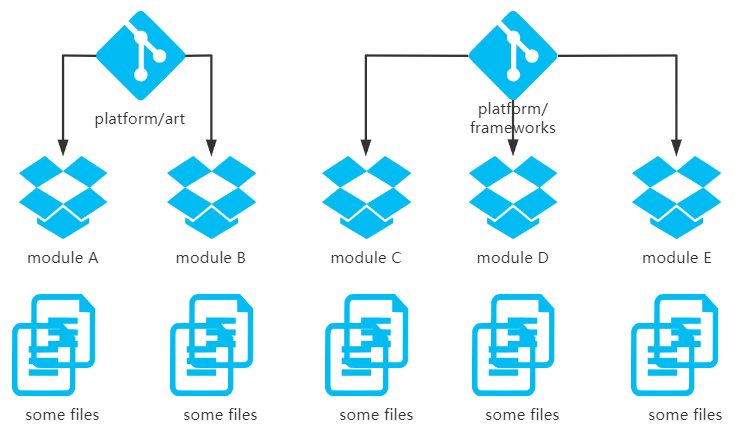
\includegraphics[width=.8\textwidth]{figures/3-layer.png}
    \caption{AOSP 三层架构}
    \label{fig:aosp-3-layer}
\end{figure}

\subsection{有向无环图}

\begin{dfn}
    给定一个有序的二元组 $<V, E>$,其中 $V$ 是一个被称作 “顶点集” 的非空有穷集。$\forall v \in V$, $v$ 被称作 “顶点”。当 $E$ 是笛卡尔积 $V \times V$ 的有穷多重子集时,$\forall e \in E$,$e$ 被称作 "有向边"。\cite{DISCRETEMATH}
\end{dfn}

\begin{dfn}
    设 $D = <V, E>$ 为有向图,$e_k = <v_i, v_j> \in E$,称 $v_i, v_j$ 为 $e_k$ 的端点,$v_i$ 为 $e_k$ 的始点,$v_j$ 为 $e_k$ 的终点。\cite{DISCRETEMATH}
\end{dfn}

\begin{dfn}
    设 $D = <V, E>$ 为有向图,$\forall v \in V$,称 $v$ 作为边的始点的次数为 $v$ 的出度,记作 $d^+(v)$,称 $v$ 作为边的终点的次数为 $v$ 的入度,记作 $d^-(v)$。
\end{dfn}

根据定义,图中有两类基本元素:节点可以用于抽象现实生活中的具体事物;边可用于抽象节点间的关系。有向图中通常使用有向边来表示节点间的偏序关系,以 $v_i$ 为始点,$v_j$ 为终点的边 $e$ 表示 $v_i \prec v_j$。而通过基于图的拓扑排序算法,可以得到有向图中一系列节点间的偏序关系集合。

\begin{dfn}
    给定一个有向图 $D = <V, E>$,其拓扑排序(见算法 \ref{alg:topology-sort})是它的顶点的线性排序。若图中存在两顶点 $v_i, v_j \in V$,则存在一条有向边 $e \in E$,且 $e$ 以 $v_i$ 为始点,$v_j$ 为终点,则记该有向边为 $e_{u v}$。在拓扑排序中,$i$ 在 $j$ 之前。
\end{dfn}

根据拓扑排序算法的定义,该算法包含了图中节点关系问题的解决方案。拓扑排序可被应用在调度任务上——图中节点被用于表示任务、图中有向边被用于表示任务间依赖关系。如果任务 $i$ 必须在任务 $j$ 开始之前完成,则存在一条从 $v_i$ 到 $v_j$ 的边。

对于任务调度问题而言,单一任务在调度全过程中只出现一次。也就是说,给定一个任务 $i$,其入度 $d^+(v_i) \le 1$,但不对其出度 $d^-(v_i)$ 做限制。由此可得,所有入度为 0 的节点 ${v'}_k \in V, (d^+(v_k) = 0)$ 是可以立即执行的任务。

\begin{dfn}
    设 $D = <V, E>$ 为有向图,$D$ 中顶点与边的交替序列 $\varGamma = v_{i_0} e_{i_0 i_1} v_{i_i} ... v_{i_{k-1}} e_{i_{k-1} i_k} v_{i_k}$ 称作节点 $v_{i_0}$ 到节点 $v_{i_k}$ 的通路。若 $v_{i_0} = v_{i_k}$,则称其为回路。
\end{dfn}

此外,为满足单一任务仅仅被执行一次,图中任意一个节点 $v_k \in V$,都不应存在一条回路。满足以上性质的图被称作有向无环图(如图\ref{fig:dag}所示)。

\begin{figure}
    \centering
    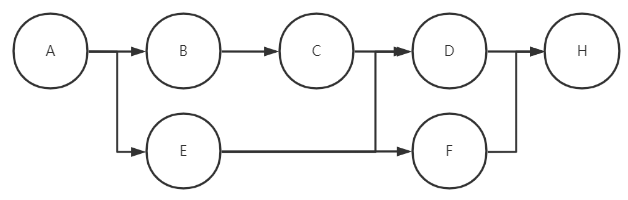
\includegraphics[width=.7\textwidth]{figures/dag.png}
    \caption{有向无环图示例}
    \label{fig:dag}
\end{figure}

\renewcommand{\thealgorithm}{2}
    \begin{algorithm}
        \caption{有向图拓扑排序算法}
        \begin{algorithmic}[1]
            \Require 输入有向图 D = <V, E>
            \Ensure 有向图是否有环
            \State initialize $q$ as a queue // 初始化队列
            \For{$i = 1 \to n$}
                \If{$D.E[i].indegree = 0$}
                    \State $q \Leftarrow E[i]$
                \EndIf
            \EndFor
            \While{$q$ is not empty}
                \State $temp \Leftarrow$ first element in $q$
                \For{$i = 1 \to n$}
                    \If{$(V_{temp} \to V_{i}) \in D.E$}
                        \State $D.E[i].indegree \Leftarrow D.E[i].indegree - 1$
                        \If{$D.E[i].indegree = 0$}
                            $q \Leftarrow D.E[i]$
                        \EndIf
                    \EndIf
                \EndFor
            \EndWhile
            \State \Return $C_1, C_2$ //输出结果
        \end{algorithmic}
        \label{alg:topology-sort}
    \end{algorithm}

结合有向图拓扑排序算法,可易得引理\ref{lem:dag}。

\begin{lem}
    一个有向图 $G = <V, E>$ 是无环的当且仅当对其进行的深度优先搜索不产生后向边。\cite{DBLP:books/daglib/0023376}
    \label{lem:dag}
\end{lem}

然而不足的是,拓扑排序受到有向图定义的限制,一条边仅能够连接始点与终点两个节点。这一缺陷降低了简单有向图对实际问题的抽象能力,下一小节将拓展现有有向图概念,使之具备描述构建系统中构建过程的能力。

\subsection{完全构建过程}

对于一个构建系统而言,其用于描述完全构建过程的 manifest 中定义了一系列独立构建过程的集合 $B$。对于单一过程 $b \in B$,其具备输入文件 $f_{in}$ 以及输出文件 $f_{out}$,可将该过程记为 $b_{<f_{in}, f_{out}>}$。若将所有输入输出文件的并集 $\bigcup_{b_{<f_{in}, f_{out}>} \in B} (f_{in} + f_{out})$ 记作 $F$,则 manifest 中定义的完全构建过程可被表示为 $P = <F, B>$。

由有向图概念可知,完全构建过程 $P$ 是一种扩展了 “边” 概念的有向图。在有向图中,$E$ 是顶点集 $V$ 的笛卡儿积 $V \times V$ 的有穷多重子集。而在完全构建过程中,$B$ 是文件集合 $F$ 非空子集 $f \subseteq F\ and\ f \neq \emptyset$ 的笛卡儿积 $f \times f$ 的有穷多重子集。后称满足上述性质的数据结构为 “扩展有向图”(如图\ref{fig:build-process}所示)。

\begin{figure}
    \centering
    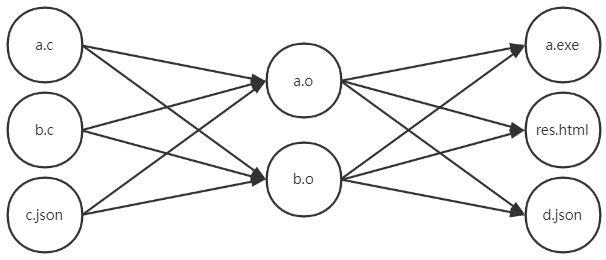
\includegraphics[width=.7\textwidth]{figures/build-process.png}
    \caption{构建过程示例}
    \label{fig:build-process}
\end{figure}

基于对项目构建的概念理解,完全项目构建具有以下特性。

\begin{enumerate}
    \item 构建过程涉及的文件数目是有限的。
    \item 构建过程是有限的。
    \item 正常的构建过程是可终止的。
    \item 出现在构建过程中的文件,其生成方式不超过一种,即:某文件不可能同时被两种方法生成。
\end{enumerate}

由有向图概念,同理可得完全构建过程 $P = <F, B>$ 的对应概念。

\begin{lem}
    给定一个完全构建过程 $P = <F, B>$,其中 $V$ 与 $B$ 是有限集。
\end{lem}   

\begin{lem}
    给定一个完全构建过程 $P = <F, B>$,定义对其中单一构建过程之间的 “拓扑排序” 为完全构建过程 $P$ 中所涉及文件集合 $F$ 的线性排序。规则为:若图中存在两顶点 $f_i, f_j \subseteq F$,则存在一条有向边 $b \in B$,且 $b$ 以 $f_i$ 为始点,$f_j$ 为终点,则记该有向边为 $b_{<f_i, f_j>}$。在拓扑排序中,$f_i$ 中所有文件 $f' \in f_i$ 在 $f_j$ 中所有文件 $f'' \in f_j$ 之前。
\end{lem}

由于对项目构建过程是可自行终止的,所以对完全构建过程 $P = <F, B>$ 进行拓扑排序可根据有向图拓扑排序算法扩展为算法 \ref{alg:total-build-topology-sort}。

\renewcommand{\thealgorithm}{3}
    \begin{algorithm}
        \caption{完全构建过程的拓扑排序算法}
        \begin{algorithmic}[1]
            \Require 输入完全构建过程 P = <F, B>
            \Ensure 完全构建过程是否有环
            \State initialize $q$ as a queue // 初始化文件队列
            \For{$i = 1 \to n$}
                \If{$D.E[i].indegree = 0$}
                    \State $q \Leftarrow E[i]$ // 获取所有源文件
                \EndIf
            \EndFor
            \While{$q$ is not empty}
                \State $temp \Leftarrow$ first element in $q$
                \For{$b \in temp.outEdges$}
                    \For{$f \in b.outputFiles$}
                        \If{$f \in q$}
                            \State \Return false
                        \EndIf
                        \State $q \Leftarrow f$                         
                    \EndFor
                \EndFor
            \EndWhile
            \State \Return true
        \end{algorithmic}
        \label{alg:total-build-topology-sort}
    \end{algorithm}

\subsection{Ninja 中对构建过程的描述}

为提供一个高效的指令执行环境,Ninja 定义了一套不同于 Makefile 的 manifest 语法(由于 Ninja 的 manifest 文件以 “ninja” 作为后缀,此后使用 ninja 代指这套 manifest 语法)。

相较于 Makefile,ninja 去除了诸如 “分支语句”、“过程定义”、“变量覆写” 等复杂语法,极大地降低了 Ninja 构建系统在运行时所需工作。ninja 专注于简洁地叙述构建过程,其语法能够最为简单地描述构建过程。

ninja 使用 “rule” (后文称为 “规则”)定义有向无环图中的边类型。在规则中,需要定义具体执行的语句,同时放置输入输出参数到恰当位置中。在规则被调用时,输入文件会被传入,同时生成符合要求的输出文件。除执行语句外,在规则语法中还可以定义最大线程数等参数进行优化。ninja 中的规则支持多输入文件到多输出文件的映射,且输入文件按照是否直接出现在执行语句中被分为 “直接依赖”、“间接依赖” 以及 “order only 依赖” 三种。ninja 使用 “build” (后文称为 “构建”)声明并实例化有向无环图中的边。ninja 格式的文件中定义了一系列构建(以 soong 构建系统产物之一 build.ninja 为例,其中使用了 90\% 以上文本描述构建)。构建是规则的实例化表现形式,其需要指定所使用的规则名,并给出规则内语句执行时需要的具体输入文件。

\subsection{模块间分析算法}

作为本文所设计软件变更分析系统的一部分,模块间分析需要根据发生变更的文件得出该变更可能影响的所有文件。

在有向图中,根据给定数量的节点搜索可达路径上所有节点的问题被称作 “多源可达问题”。然而,模块间分析并不完全等价于 “多源可达问题”。基于 Ninja 构建系统定义的完整构建过程 $P = <F, B>$ 以及实际构建过程中模块间的影响,模块间影响可分为以下两种情况。

\begin{enumerate}
    \item 文件 $a$ 改变,$\exists\ b_{<f_{in}, f_{out}>} \in B$,且文件 $a \in f_{in}$,$f_{out}$ 中所有文件受到直接影响,而 $f_{out}$ 可能被认定属于其他模块。如图\ref{fig:inter-module}中 a.2 对 a.3 的影响。
    \item 文件 $a$ 改变,$\exists\ b_{<f_{in}, f_{out}>} \in B$,且文件 $a \in f_{in}$,$f_{in}$ 中所有除 $a$ 之外的文件都可能因 $a$ 的改变而受到间接影响,而 $f_{in}$ 中其他文件可能来自于其他模块。如图\ref{fig:inter-module}中 a.2 对 sub.3 与 sub.4 的影响。
\end{enumerate}

\begin{figure}
    \centering
    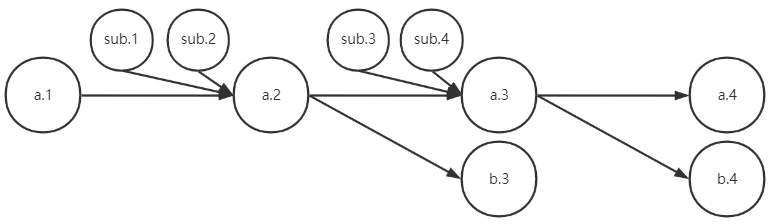
\includegraphics[width=.8\textwidth]{figures/inter-module.png}
    \caption{模块间影响示意图}
    \label{fig:inter-module}
\end{figure}

在传统有向图中,“多源可达问题” 可使用图搜索算法解决。而在扩展有向图中,上述结论仍旧成立。对于深度优先搜索算法与广度优先搜索算法,在解决该问题时,存在以下可供权衡的观点。

\begin{itemize}
    \item 深度优先搜索是求解 “多源可达问题” 的最通用算法。然而在构建问题背景下,很难通过深度优先算法获得必要的构建次序信息。
    \item 广度优先搜索通过维护文件队列搜索扩展有向图。然而 AOSP 的体量庞大,需要大量单元表示文件状态。
\end{itemize}

为获取有关构建过程的更多信息,本文所设计的软件变更分析系统采用广度优先搜索,如算法\ref{alg:intermodule-analysis}所示。综上所述,在扩展有向图 $P = <F, B>$ 中搜索可能受影响文件的本质仍是图可达性问题,该问题仍可在 $O(F + B)$ 中解决。\cite{GRAPHREACHABILITY}

\renewcommand{\thealgorithm}{4}
    \begin{algorithm}
        \caption{基于 Ninja 的过程间分析算法}
        \begin{algorithmic}[1]
            \Require 输入完全构建过程 $P = <F, B>$
            \Require 输入被修改的文件集合 $F_{in}$
            \Ensure 被直接影响的文件集合 $F_{direct}$
            \Ensure 被间接影响的文件集合 $F_{indirect}$
            \State initialize $q$ as a queue // 初始化文件队列
            \For{$f_{in} \in F_{in}$}
                \State $q \Leftarrow f_{in}$
                \State $F_{direct} \Leftarrow f_{in}$
            \EndFor
            \While{$q$ is not empty}
                \State $temp \Leftarrow$ first element in $q$
                \State $outputFiles \Leftarrow$ get all output files by $temp$
                \For{$f \in outputFiles$}
                    \If{$f \notin F_{direct}$}
                        \State $q \Leftarrow f$
                        \State $F_{direct} \Leftarrow f$
                    \EndIf
                \EndFor
            \EndWhile
            \For{$fd \in F_{direct}$}
                \State $inputFiles \Leftarrow$ get all input files by $fd$
                \For{$f \in inputFiles$}
                    \If{$f \notin F_{direct}$}
                        \State $F_{indirect} \Leftarrow f$
                    \EndIf
                \EndFor
            \EndFor
            \State \Return $F_{direct}, F_{indirect}$
        \end{algorithmic}
        \label{alg:intermodule-analysis}
    \end{algorithm}
